\documentclass[fontsize=11pt]{article}
\usepackage{amsmath}
\usepackage[utf8]{inputenc}
\usepackage{amsmath}
\usepackage[utf8]{inputenc}
\usepackage[margin=0.75in]{geometry}
\usepackage{hyperref}
\usepackage{graphicx}
\hypersetup{
    colorlinks=true,
    linkcolor=blue,
    filecolor=magenta,      
    urlcolor=blue,
}

\usepackage{setspace}
\usepackage{tabularx}
\usepackage{hyperref}
\usepackage{parskip}


\title{CSC111 Final Project: Comparing and Mapping Wikipedia's Articles}
\author{Gabe Guralnick, Matthew Toohey, Nathan Hansen, Azka Azmi}
\date{Friday, April 16, 2021}

\begin{document}

\maketitle

\section{Background}

Wikipedia is an online encyclopedia used by millions of people to learn just about anything. From quick look-ups to in-depth research, it can be an excellent tool for finding information. 

Wikipedia sorts its articles into various topics and categories. These categories range from sweepingly broad to very specific. Take, for example, the page about William Clark (whom you may know from the Lewis and Clark expedition). His article falls under the categories \textit{United States Army Officers}, a very large category, as well as \textit{People from Caroline County, Virginia}, which is significantly smaller. Wikipedia articles also have many subcategories, creating a hierarchical structure. For example, the \textit{People from Caroline County, Virginia} category is a subcategory of the \textit{People by county in the United States} category.

But in an age of seemingly limitless information easily accessible over the Internet, it becomes difficult for casual users to determine what information is ``worth'' learning: which topics are actually influential and important, and which ones are more in the background?

Wikipedia itself does not differentiate between the ``importance'' of each of its articles. This approach is helpful in preventing any sort of discrimination on their part, but it prevents users from getting an idea of what people, places, or events are the most influential in human history. Because of this, for our project, we hope to create a system for determining what topics are the most important.

This is a difficult question to answer, however; you could say that ``United States'' would be a very important article due to the country's large-scale involvement in global politics, but from an astronomer's perspective it's not very relevant. For this reason, our goal is for our solution to be user-driven: any user of our program will be able to input the category that they're interested in, and then our program will determine the most important topics within that category.

There are several possibilities for criteria as to the influence of a given topic. One is how frequently its article is referenced by others on Wikipedia. Intuitively, if an article is linked too often by other articles, and links to many other articles, it is probably more influential, of higher quality, and more useful. Another, slightly more complicated criteria is a sorting algorithm like Google's PageRank, which considers the number of links not just of a given page, but of the pages that link to it as well (Wikipedia contributors, 2021). PageRank models the probability that a web surfer clicking links randomly will arrive at a given page. As mentioned before, since Wikipedia contains a massive amount of different articles and topics, we'll focus on a given (user-selected) category. For our project, we will investigate this research question:

\noindent \textbf{What are the most important or influential articles across Wikipedia pages of a given category?}

%###########
\section{Computational Overview}

The core of our program is the Python \texttt{wikipedia-api} library, which accesses the Wikipedia API. This library allows us to create \texttt{WikipediaPage} objects based on article titles. These objects are initialized using an article/category title and have various
properties including links, back-links, and categories, which will all be vital in allowing us to model the
relationships between articles and categories. These properties are exactly what their names suggest: the links
property provides a dictionary of titles to the related \texttt{WikipediaPage} objects that linked to by this article, back-links
is a similar dictionary except that it includes articles that link to this page, and categories is another dictionary
containing the categories the article belongs to. All of this functionality is essential to answer our project question.
The first step in our computation occurs in the \texttt{wiki\_graph} module, with the \texttt{create\_digraph} function. This function receives a Wikipedia category as a parameter and returns a \texttt{networkx.DiGraph}. Each vertex in the graph represents a Wikipedia article in the category, and each directed edge represents a link from one article to another. Although we could have used our graph implementations from lectures and assignments, we wanted the additional functionality provided by \texttt{networkx}, like visualization algorithms and directed edges.
Next, our program moves into the \texttt{algorithms.py} modules. The functions in this file, which all serve to calculate the PageRank scores of each article in the category, are called by other functions in our \texttt{recommendations.py} and \texttt{visualize.py} modules. 
First, there is \texttt{calculate\_pagerank}, which takes a \texttt{networkx.Graph} as a parameter, calls the \texttt{networkx.algorithms.link\_analysis} implementation of the PageRank algorithm, and returns a dictionary with article titles as keys and PageRank scores as values. This method produces satisfactory results for the purposes of our visualizations and recommendations, but we wanted to go more in-depth with the algorithm itself, and so decided to implement our own version of PageRank, contained in \texttt{calculate\_pagerank\_manual}.
A simplified version of the algorithm is as follows: Let \(A, B, C, D\) be the pages under consideration. Suppose \(B, C, D\) all link to \(A\). Then the PageRank score for \(A\) is the sum of the PageRank scores of \(B, C\), and \(D\), each divided by the number of outbound links on that site. In other words,
$$PR(A) = \frac{PR(B)}{L(B)} + \frac{PR(C)}{L(C)} + \frac{PR(D)}{L(D)}$$
where \(L(i)\) is the number of outbound links from a given page \(i\) to other pages under consideration.
In general, if \(P\) is an arbitrary page and \(I\) is the set of pages that link to \(P\) (note the inbound direction, links from \(P\) are not included here), then
$$PR(P) = \sum_{i \in I} \frac{PR(i)}{L(i)}.$$ Additionally, if a given page has no outbound links, its PageRank score is distributed over the rest of the pages in the set of all pages; if \(p\) is such a ``dangling'' page, then \(\frac{PR(p)}{N}\) is added to the scores of all pages in the set, with \(N\) the total number of pages under consideration. Our implementation also considers a ``damping'' factor \(d\), to reflect the fact that a person clicking links randomly will eventually stop, so the true calculation, with \(D\) representing the set of dangling pages, is
$$PR(P) = \frac{1-d}{N} + d\sum_{i \in I} \frac{PR(i)}{L(i)} + d \sum_{p \in D} \frac{PR(p)}{N}$$
PageRank scores are computed iteratively: in the first iteration, each page is assigned a score of \(\frac{1}{N}\), then the calculations described above are repeated until the scores for each page converge over successive iterations.
Our implementation of this algorithm differs from the \texttt{networkx} implementation, which uses various linear algebra concepts to represent PageRank scores as a matrix and uses a power iteration method to compute scores. We wanted to include both to see how the two methods differ in complexity and results, and to get a better understanding of how the algorithm works. Theoretically, they should produce the same results, though in our case the two methods differ slightly, which will be discussed in our limitations section. \texttt{calculate\_pagerank\_manual} also returns a list of dictionaries, rather than a single dictionary, as the results from each iteration are used in \texttt{visualize\_convergence}.

The \texttt{visualize.py} file provides various options for visualizing the resulting data produced by the algorithms we have just discussed. They all make heavy use of the \texttt{plotly} module. Most directly related to the implementation of PageRank discussed in the previous paragraph is the \texttt{visualize\_convergence} function. This method calls \texttt{calculate\_pagerank\_manual} and uses the resulting dictionaries to create one line trace for each article in the graph, which are then displayed on a line graph. These line graphs demonstrate how the PageRank score of each article changes on each iteration of the algorithm.

The next set of functions display visualizations of a graph, in a style similar to our graphs from A3. The \texttt{visualize} method is a helper method that handles much of the necessary leg-work for adding the lines (or arrow annotations) and nodes of a graph and is used by both the \texttt{visualize\_digraph} and \texttt{visualize\_pagerank} functions. The \texttt{visualize\_digraph} function displays a simple diagram of a given \texttt{graph} object, optionally using lines that make the graph less cluttered, or arrows that indicate the directions of the links. However, all the nodes have uniform sizes. \texttt{visualize\_pagerank} displays a similar visualization, but with an added layer of information: nodes have different sizes based on their computed PageRank scores. Information regarding the page title, exact PageRank score, as well as the number of local and global links and back-links, are all displayed in tool-tips that appear when a node is hovered over. In terms of their implementation, both of these functions use the \texttt{networkx.spring\_layout} function to convert the provided graph to a set of positions, then they use the nodes of the provided graph to create the edges, labels, and coordinate lists that must be passed to the \texttt{visualize} function.

The final visualization function creates a histogram displaying the distribution of local links (links to other pages within the categories) and back-links for pages within the provided graph's category, or alternatively, displays the total links and back-links, not just the local ones. This function makes use of the \texttt{assign\_link\_stats} function in the \texttt{algorithms.py} file, which assigns the different link metrics to each node as an attribute. Then the function uses a comprehension over the graph's nodes to aggregate these values into lists that are fed into a Plotly histogram. Finally, various aesthetic properties of the graph are adjusted, most notably the bin groups, so that both the links and back-links are shown with the same bin widths.

The file \texttt{recommendations.py} takes heavy inspiration from the computational methods we learned back in A3, which implemented various recommendation systems through the use of similarity scores. There are three distinct recommendation systems within this file. Computationally they all behave in a similar manner, yet produce distinctive results. Recall that the similarity score used by A3 determines how similar two nodes are to each other by assigning them a similarity score that is calculated by dividing the number of neighbours they share by the total number of neighbours either of them have. Our function \texttt{similarity\_score} uses this same algorithm in order to determine how similar two pages within our \texttt{networkx} Wikipedia graph are to one another. This similarity score is then used within \texttt{top\_wiki\_page\_recommendations}, which takes a page that exists in our \texttt{networkx} graph, calculates its similarity score between itself and all other pages within the graph and then returns the top pages with the highest score. 

Our last two recommendation systems behave in a slightly different manner. \texttt{top\_wiki\_pages} is a function that aims to return the top \(n\) Wikipedia pages within an inputted networkx graph. It takes a more basic and straightforward approach to what it considers the ``top'' pages within a category and relies heavily on \texttt{networkx} graph principles. \texttt{top\_wiki\_pages} considers pages with the most number of adjacent pages to be ``top'' ranked pages within their category. It uses a basic traversal pattern to loop through each node within the graph in order to unpack each node and its number of neighbours into a separate list of tuples. It then uses the filtering and sorting function, \texttt{reverse\_list\_sort}, to return the ``top'' pages with the \texttt{networkx} graph. \texttt{top\_wiki\_pagerank\_pages} computationally differs from the above algorithm as it defines its ``top'' pages through the use of \texttt{PageRank's} scores of importance. As explained previously, we know that \texttt{PageRank} assigns each page within its graph an importance score by calling the function \texttt{algorithms.link\_analysis.pagerank()} onto a graph object. Using this definition, the function, \texttt{top\_wiki\_pagerank\_pages} then defines the ``top'' pages within a category to be based around these scores and returns its recommendation list as such. The function, \texttt{wiki\_link\_pages} is a helper aggregation method that takes in a list of page names and uses Wikipedia's API to determine the URLs of each page name by calling, \texttt{fullurl()} onto a page object. It then returns a list of tuples that contain the page name as its first element and its successive URL as the second. 

All of these functions and recommendation systems are then used within 2 distinct visualizations within our program. \texttt{visualize\_recommendation} takes in a \texttt{networkx} graph and a page that exists within that graph, and uses Plotly's graphing modules and libraries to represent a table of Wikipedia page recommendations, their URLs and their similarity scores. This visualization produces these results from our recommendation function, \texttt{top\_wiki\_page\_recommendations}, and aggregation function, \texttt{wiki\_link\_pages}. The second visualization, \texttt{visualize\_rankings}, takes in a category name and uses the remaining two recommendation algorithms, \texttt{top\_wiki\_pagerank\_pages and top\_wiki\_pages} in accordance with Plotly's libraries to create a comparison visual for the user. This resulting visual displays a chart and two bar graphs that compare the results of what both recommendation systems consider to be the ``top'' ranked pages within their \texttt{networkx} graph.

%###########
\section{Instructions for Running the Program}

\subsection{Requirements.txt}

Start by installing the required modules, either through your preferred IDE's GUI or from the command line by running: \texttt{pip3 install -r requirements.txt}.

% Informing the TA on how to access all visualizations etc
\subsection{How to Interact with the Program}

\begin{enumerate}
    \item Begin by running the \texttt{main.py} file. No additional downloads are required, as the program fetches the necessary data automatically based on user input. Upon starting the program the user will be presented with a title screen and a main menu with options to choose from. Initially only menu options 1 (\texttt{Select a Category}) and 4 (\texttt{Exit}) will be  available for the user to select. Options 2 (\texttt{Category Visualizations}) and 3 (\texttt{Category Recommendations}) will not become available until after the user has completed option 1 at least once.
    \item In order to interact with the program, the user must first successfully complete the first option, which allows the user to select any type of Wikipedia category. If the category does not exist, the user will be prompted for new input until a category is finally selected. Note that it may take some time to load particularly large categories. They will then be returned to the menu screen.
    \item Once the user has accomplished the previous task, they now have access to all other options.
    \item Upon Selecting Option \texttt{2 - Category Visualizations} 
    \begin{enumerate}
        \item If the user decides to select option 2, they will then be presented with a sub-menu whose options correspond with the four types of Graphical Visualizations in our implementation.
        \item If the user chooses to select option 1 (\texttt{Visualize Graph}) they will then be presented with a \texttt{plotly} visualization depicting an interconnected \texttt{networkx} graph. The circular objects within this graph represent each page within the user's category and the lines between them represent links/edges between different pages. The visualization also uses a spring layout. The user is able to hover over distinct circles for a description of each page.
        \item If the user chooses to select option 2 (\texttt{Visualize PageRank Graph}) they will also be presented with a \texttt{plotly} visualization depicting an interconnected \texttt{networkx} graph. This graph shares many of the same properties as the one from option 1, however, this time the pages are sorted using PageRank's algorithms of page importance and a spring visual layout. By this, we mean that pages that are similar will ``attract'' one another and pages that have little to no similarity will ``repel'' each other. This gives added depth to our simulation and results in a very interesting visual. 
        
        \begin{figure}[h]
            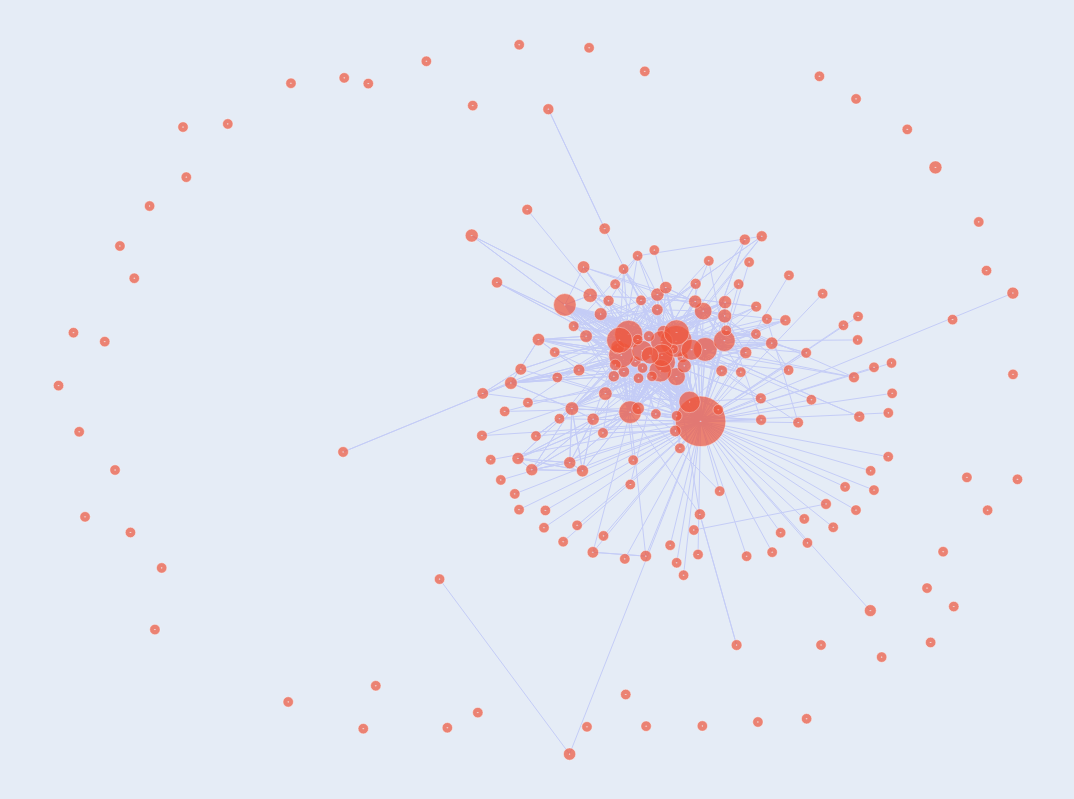
\includegraphics[scale=0.45]{Programming languages PageRank.png}
            \centering
            \caption{``Programming languages'' PageRank Graph Visualization}
        \end{figure}
        
        \item If the user chooses to select option 3 (\texttt{Visualize PageRank Convergence}), the \texttt{calculate\_pagerank\_manual} method will be used to create (and display a line graph) demonstrating how the PageRank algorithm iteratively converges to its final values.
        
        \begin{figure}[h]
            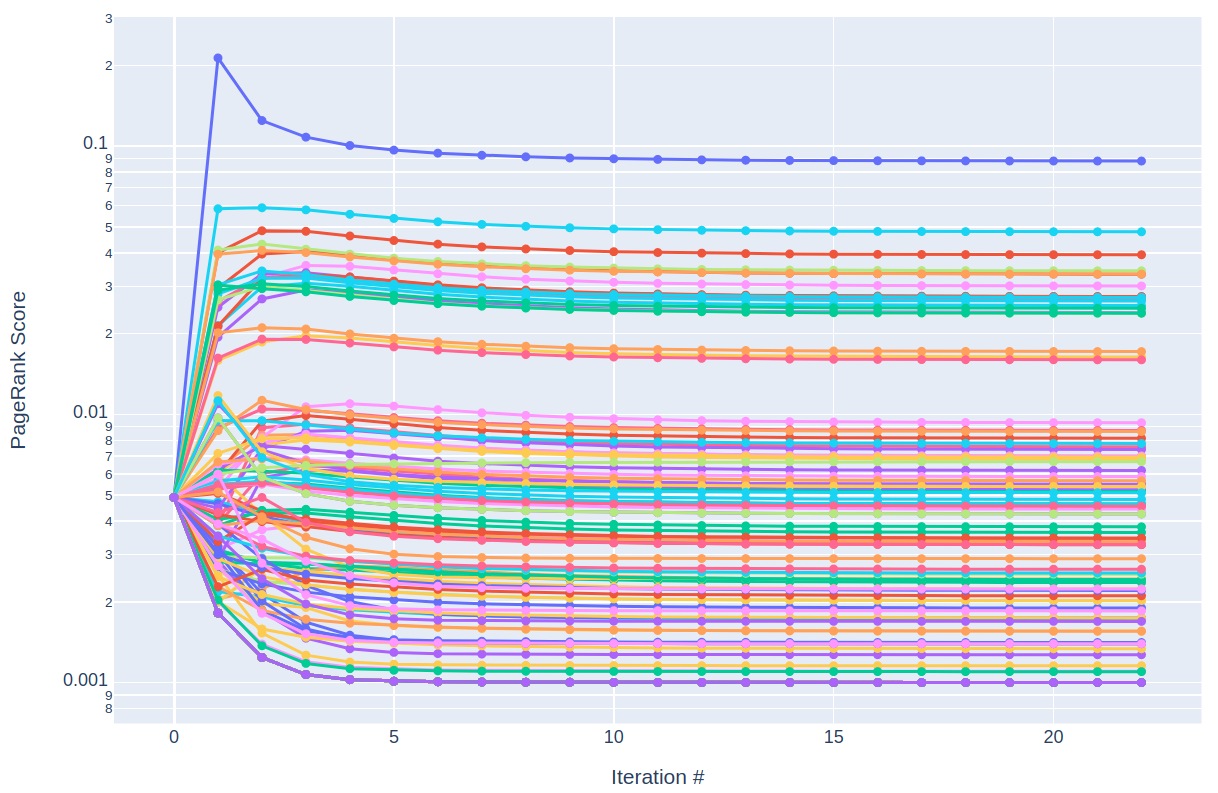
\includegraphics[scale=0.45]{Programming languages Convergence.png}
            \centering
            \caption{``Programming languages'' PageRank Convergence Visualization}
        \end{figure}
        
        \item If option 4 is selected (\texttt{Visualize Link Histograms}), the user will be presented with a histogram that displays the distribution of local links and local back-links present for the pages in the selected category. Using this histogram, the user can observe how ``concentrated'' links within a specific category are, for example, in some categories the user may observe that a specific page has far more back-links than almost all other pages in that category, whereas in others they may see that the quantities of links and back-links are more evenly distributed.
        \item NOTE: The time taken to display these simulations may vary depending on the size of the user's category. We recommend starting out with smaller-sized categories (such as ``Cats'' or ``Pastas'') to test these options before continuing. 
    \end{enumerate}
    
    \item Upon Selecting Option \texttt{3 - Category Recommendations}  
    \begin{enumerate}
        \item If the user decides to select the third option, they will first be asked to enter in a valid number of recommendations that they would like to see. Note that while a user may want to see 100 recommendations for a category, category sizes vary and resulting lists and visualizations may show less. The user will then be presented with a list of all the pages in their category and will then be asked to choose one. Note that these input statements will reoccur after every successful visualization. 
        \item If the user chooses option 1 (\texttt{List of Top Ranked Wikipedia Pages (Basic)}) or option 2 (\texttt{List of Top Ranked Wikipedia Pages (PageRank Importance)}), the program will print out a list (whose size will be less than or equal to the amount of recommendations they asked for) of top pages within their category, and its score based on the chosen algorithm. 
        \item If the user chooses option 3 (\texttt{List of Top Page Recommendations ... based on Similarity Scores}) the program will print out a list of recommendations and their similarity score based on their chosen page from their category. 
        \item If the user chooses option 4 (\texttt{Comparison Visual of Top Ranked Pages}) they will be presented with a visualization of two bar graphs and one table on the same page. The table is a comparison chart that demonstrates the top ranked pages of the user's Wikipedia category using both ranking algorithms from options 1 and 2. The First bar graph uses the basic ranking algorithm and is a representation of the pages vs connection scores. This chart will always be in terms of greatest to least. The second bar graph uses PageRank's importance algorithms to map Page names vs importance score. As these two bar graphs are on top of one another, it allows the user to easily recognize the differences in what PageRank and the Basic algorithm consider ``Top'' pages.
        
        \begin{figure}[h]
            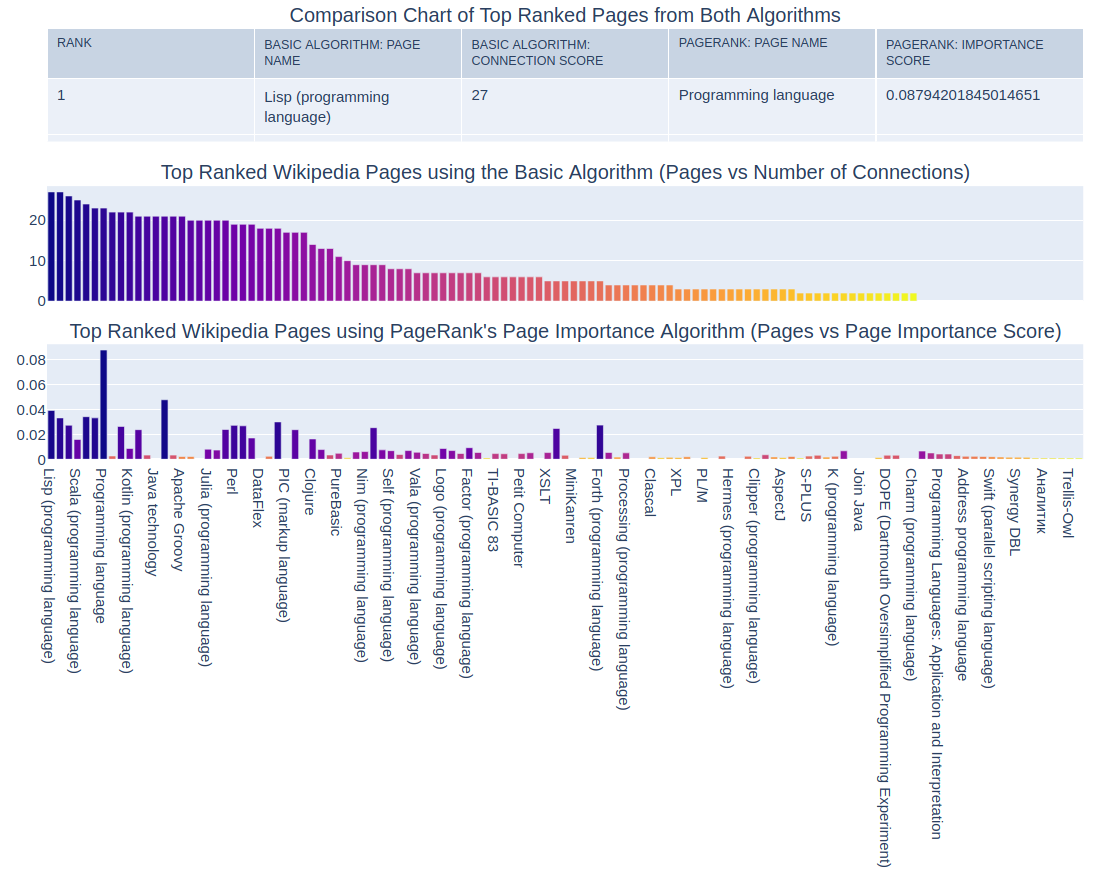
\includegraphics[scale=0.45]{Programming languages Recommendations.png}
            \centering
            \caption{``Programming languages'' PageRank Recommendations Visualization}
        \end{figure}
            
        \item If the user chooses option 5 (\texttt{Chart Visual of Top Page Recommendations ... Based on Similarity Scores}) they will be presented with a chart visual that utilizes the list in option 3 to chart top recommendations for their chosen page in their category, their similarity scores, and their URLs. 
    \end{enumerate}
\end{enumerate}

%###########
\section{Alterations From the Proposal}
\noindent The largest change in our project from the proposal is our method of sorting the articles and determining which are the most influential. Originally, we were just going to determine this based on the number of links to and from each article; when the PageRank algorithm was brought up in lecture, however, we realized that it would be the perfect algorithm to answer our project question. We still included the sorting algorithm based on the number of links, however, so that we could see how the two methods produce different results.
We were also planning to use recursion to traverse through Wikipedia articles, perhaps as part of our graph creation process. In the proposal, we noted that the incredible number of articles present on Wikipedia could mean that a recursive approach would be very computationally intensive for large categories. In the end, we realized that the \texttt{wikipedia-api} package's Wikipedia article objects contain a property \texttt{categorymembers}, which allowed us to just get a dictionary with all of the articles in a given category as elements. This was a much simpler method for constructing our graphs, and could scale much better to larger categories.
While writing the proposal, we also weren't sure whether any of the Graph methods we had created in lecture and assignments would be applicable to this problem domain, so we weren't planning on incorporating them; in the end, however, we found a use for the similarity score and book recommendation methods we had made in A3, and modified those to operate on our \texttt{networkx.DiGraph}.

%###########
\section{Discussion}
\noindent

\subsection{Results}
Recall that the research question of our program was to determine \textbf{the most important or influential articles across Wikipedia pages of a given category}. While our program hosts over 6 different implementations in order to solve this question, the resulting graphical visuals created by \texttt{networkx} and \texttt{plotly} allowed for an easily understandable and interactive answer for the user. Generally, the overarching answer to this problem relies on how one defines importance and/or influence, as the answer may vary from person to person. Does the user consider the most important Wikipedia articles to have the most links and back-links or the most connections to other articles in the same category? How exactly do we measure the importance of each page in our program? And is the most influential page the one that consistently scores high on all of our implementations? All of these are legitimate questions we must address in order to provide a general answer to our research question. That is, how does our program enable user input to answer this question for themselves. 

To give an example of one result of our research question, let us take the category: `Prolog programming language family'. The straightforward approach to determine its most `important' article would be to simply use our graph modules to visualize the category and then make determinations from there. Through the PageRank visualization we can conclude that this article would be, `Prolog,' the largest node within the graph, followed by `Comparison of Prolog Implementation' and then `SWI Prolog'. Our basic graph visualization makes this slightly harder to accomplish, however, the results are largely the same. Through visual comparison we can determine that once again, `Prolog' and `Comparison of Prolog Implementation' are still the top two, however the third most connected article is replaced by `Logtalk'. Similarly if we were to call our basic ranking algorithm to determine the `top' ranked pages within this category, we see almost the exact same results. `Prolog' is once again at the top, followed by `Logtalk' and then `Comparison of Prolog Implementation.' In this instance we can see that the top article within this category is undoubtedly `Prolog,' however the three algorithms have slightly differing results when it comes to the importance of the remaining articles. While this great amount of similarity worked out well for this category, one may not be able to say the same for various other larger ones. As such, we'd like to emphasize that the way in which our program answers our research question is through allowing the user to outline their own understanding of what defines an `important' Wikipedia article before offering them the tools to investigate the answer to that question.

Other noteworthy findings from our program arose through the use of histograms to model the distribution of links and backlinks across categories, which revealed some insights as to how Wikipedia categories tend to interlink. Using the ``Visualize Link Histograms'' function under ``Category Visualizations'' creates a graph showing the spread in the number of links or backlinks across pages in a category. Generally, most pages have few or no backlinks, and a small number of links. However, oftentimes categories will have a few pages that are visited far more frequently than others. These pages tend to have far more backlinks than the rest of their category, since other pages will link to them more than other category members. However, this does not directly correlate to having a large number of links within the article itself, which is likely a product of article length.

\subsection{Limitations}
One limitation of our program is our manual PageRank implementation. Since PageRank scores represent a probability distribution, they should, theoretically, sum to 1. The results from the \texttt{networkx} implementation of the algorithm do, but due to some simplifications made on our part the results from \texttt{calculate\_pagerank\_manual} only sum to about 0.96. We decided this was acceptable, as the results returned by both algorithms are still very similar.

Another limitation is the amount of time it takes for certain operations to run. This is mostly a limitation of the \texttt{wikipedia-api} module, since it does take some time to download all the data from large categories. One potential improvement that would mitigate this issue would be to implement a system for caching graphs that have already been created, so that they wouldn't need to be downloaded multiple times. We were able to partially resolve this issue in our \texttt{main.py} file by storing the graph and re-using it for each of the different visualizations, instead of re-creating it each time. This limitation also prevented us from studying larger collections of articles, because even moderately sized categories can take a minute or two to download.

\subsection{Further Exploration}

One thing we discussed while working on this project was modelling Wikipedia pages beyond a single category. We found that Wikipedia categories tend to have a hierarchical structure, with sub- and super-categories. A possible extension, then, of our project could be modelling these relationships between categories as a tree and visualizing them in that fashion.

If we wanted to improve upon the current recommendations system, one possibility would be adapting our current system so that it learns from a user's input. As the user asks for more wiki articles, the system could use their previously selected articles to compute a similarity score based on multiple articles.

Another similar algorithm that we considered looking into, but didn't end up implementing, is the HITS algorithm for ranking pages. This algorithm ranks the ``authority'' of pages, though since it is based on the idea of ``hubs'' which link to multiple other sites, it may not be as directly applicable to Wikipedia as PageRank.

\subsection{Conclusion}

Over the course of this project, our group has investigated the connectivity of Wikipedia articles in a multitude of ways, with the core utility of the graph serving as a backbone for our research. In our research question, we wondered what factors make a Wikipedia article important to a category. As it turns out, the articles that perform best in \texttt{pagerank} algorithms could not do so without the neighbouring articles in their category. If nothing else, this project has shown that the community-driven ideals that Wikipedia was built on extend down to the very links that hold the site together.


\newpage

%###########
\section*{References}

% NOTE: LaTeX does have a built-in way of generating references automatically,
% but it's a bit tricky to use so we STRONGLY recommend writing your references
% manually, using a standard academic format like APA or MLA.
% (E.g., https://owl.purdue.edu/owl/research_and_citation/apa_style/apa_formatting_and_style_guide/general_format.html)

\noindent Majlis, M. (n.d.). Wikipedia-API: Python Wrapper for Wikipedia. PyPI. \href{https://pypi.org/project/Wikipedia-API/}{https://pypi.org/project/Wikipedia-API/}

\noindent Network Graphs. (n.d.). Plotly.com. \href{https://plotly.com/python/network-graphs/}{https://plotly.com/python/network-graphs/}

\noindent NetworkX — NetworkX documentation. (n.d.). Networkx.org. \href{https://networkx.org/}{https://networkx.org/}

\noindent Wikipedia contributors. (n.d.). PageRank. In Wikipedia, The Free Encyclopedia. Retrieved April 12, 2021, from \href{https://en.wikipedia.org/wiki/PageRank\#Simplified\_algorithm}{https://en.wikipedia.org/wiki/PageRank\#Simplified\_algorithm}

\noindent Wikipedia contributors. (2021, March 13). William Clark. In Wikipedia, The Free Encyclopedia. Retrieved March 15, 2021, from \href{https://en.wikipedia.org/w/index.php?title=William_Clark&oldid=1011838536}{https://en.wikipedia.org/w/index.php?title=William\_Clark\&oldid=1011838536}

\end{document}
